\documentclass{article}
\usepackage[utf8]{inputenc}
\usepackage{graphicx}
\usepackage{float}
\usepackage{listings}
\usepackage[margin=1in]{geometry}

% Preamble 
    \title{Project 01: Networking}
    \author{Courtney Kelly, Katie Schermerhorn, Ben Dalgarn}
    \date{April 20, 2016}

% Document Body 
    \begin{document}
    
    \maketitle
    
    \section*{Summary}
    
    In this project, we successfully created a HTTP client and a HTTP server.  In thor.py, we created a program that dials into the server and makes a request.  Spidey.py is a program that listens for connections and processes them.  In order to do this within a group, we used BitBucket.  If any of us were to make changes, we would commit and push them to the repository.  The majority of the work was done all together using paired programming. We found that it was unsuccessful to code separately because if someone would make changes, the others would fall behind in understanding and the person who made the changes would have to take the time to bring the rest of the group up to speed. It was more efficient if we all coded together, each of us coming up with different ideas to solve problems.
    \newline
    \newline
    We ran into some difficulties when parsing the request in the server (spidey.py).  We fixed these problems by using the verbose mode with debugging enabled to see when in the program we ran into problems and by printing all of our parsed variables to check their accuracy. We had the most trouble with the hello.sh script. When you first clicked on the script, our program would interpret the html correctly. However, when we tried to run the script with a name it would fail. We identified the problem with the help of Dr. Bui, would explained we weren't parsing our "REQUEST URI" environment variable incorrectly: it was including the query string when it shouldn't!
    
    \section*{Latency}
    To measure the latency of the requests, we used two shell scripts which ran thor.py and spidey.py. In one shell script - test_latency.sh, we ran thor.py with 10 processes and 10 requests each for directory listings, a static file, and a CGI script.  We then filtered the output into grep to get all of the lines with "Average".  This collected the average elapsed time of each process.  From there, we piped this into cut to filter out all of the words.  Then, we used awk to add all of the times of the 10 processes and average them into one.  In the other shell script - test_latency_spidey.sh, we ran two instances of spidey.py: one in forking mode and one not.  This script was run before the other.  The thor.py shell script was run with matching ports to connect it to the server we developed. 
    
        % Latency Table
        \begin{table}[H]
            \centering
            \begin{tabular}{c|c|c}
            \hline
                {\bf HTTP Request} & {\bf Single Connection} & {\bf Forking Mode} \\
            \hline
                Directory Listings & 0.071 & 0.062 \\
                Static Files & 0.083 & 0.072 \\
                CGI Scripts & 0.135 & 0.15 \\
            \hline 
            \end{tabular}
            \caption{Latency of Single Connection vs. Forking Mode}
            \label{tab:latency_table}
        \end{table}
        
        % Latency Graph
        \begin{figure}[H]
            \centering
            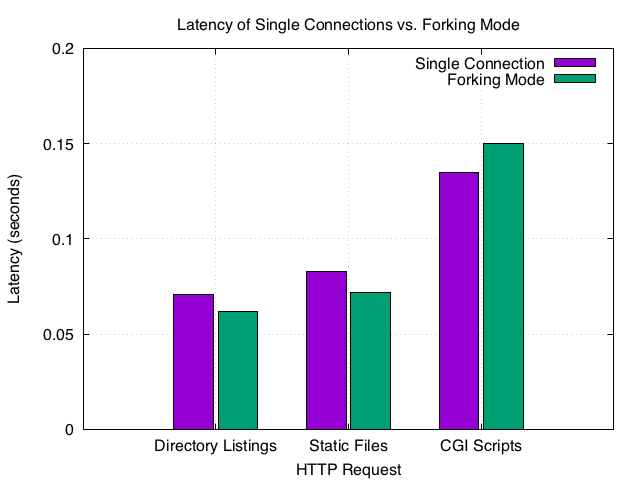
\includegraphics[height=4in]{latency.png}
            \caption{Latency Histogram}
            \label{fig:latency_graph}
        \end{figure}
    
    \section*{Throughput}
    We calculated throughput very similarly to the way we calculated latency.  We did the same commands, but only allowed thor.py to run one request and one process.  Instead of running in one for different kinds of directories and files, we ran it on different sizes of static files.  We made three static files of different sizes (1Kb, 1Mb, and 1Gb) using the command 'dd'.  We then ran the scripts which outputs the average elapsed time for each of the different sized files.
        
        % Throughput Table
        \begin{table}[H]
            \centering
            \begin{tabular}{c|c|c|}
            \hline
                {\bf HTTP Request} & {\bf Single Connection} & {\bf Forking Mode} \\
            \hline
                Small Static File (1k) & 0.12 & 0.07  \\
                Medium Static File (1M) & 0.12 & 0.15 \\
                Large Static File (1G) & 88.7 & 65.4 \\
            \hline 
            \end{tabular}
            \caption{Throughput of Single Connection vs. Forking Mode}
            \label{tab:throughput_table}
        \end{table}
        
        % Throughput Graphs
        \begin{figure}[H]
            \centering
            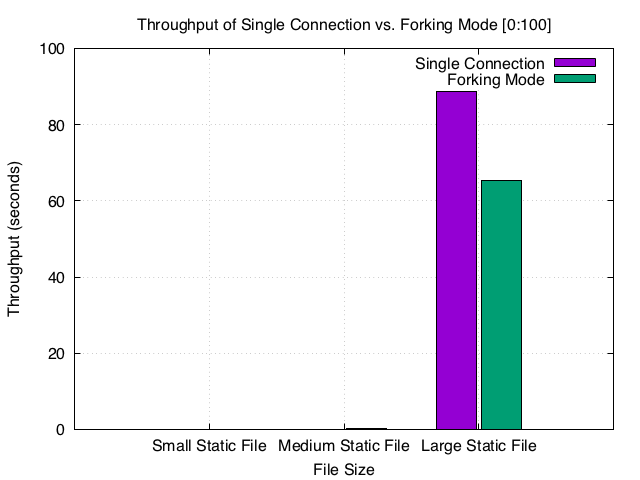
\includegraphics[height=4in]{throughput1.png}
            \caption{Throughput Histogram: Range 0-100}
            \label{fig:throughput_graph}
        \end{figure}
        
        \begin{figure}[H]
            \centering
            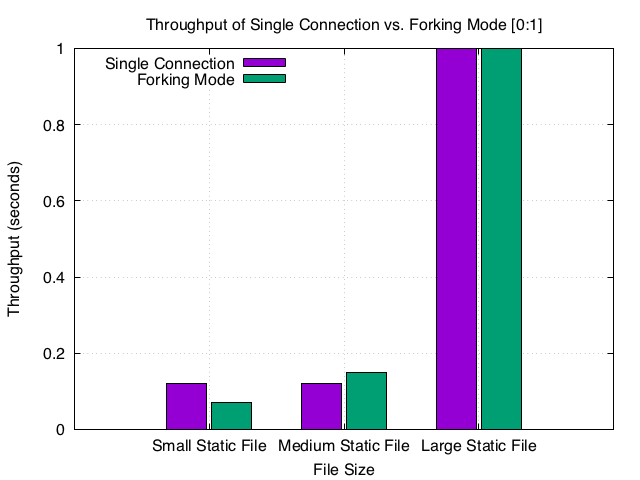
\includegraphics[height=4in]{throughput2.png}
            \caption{Throughput Histogram: Range 0-1}
            \label{fig:throughput_graph}
        \end{figure}
    
    \section*{Analysis}
    Our experiment determined that forking mode had a lower latency the majority of the time.  In the case of directory listings and static files, forking is faster.  This is not the case, however, for CGI scripts.  Our experiment also determined that the throughput for forking mode was also lower.  Forking mode and non-forking had similar throughputs for both small and medium files.  We see a big difference when looking at the throughput of the large static file.
    
    We received these results, because forking handles multiple concurrent requests better than non-forking.  When there are multiple requests and processes, the forking should lessen the latency.  The same goes for throughput.
    
    
    \section*{Conclusions}
    From the lab assignment as a whole, we learned how machines communicate with one another. When we type in a URL in our browser and push enter, our machine is making a GET request. It's requesting the html code from the machine that corresponds to that domain/IP address (name resolution). The machine that receives this request will then parse and process it, and send back another message, usually 200 OK or 404 Error. This all occurs through Networks and is possible because of these things called sockets. When you make a GET request the first thing you do is instantiate a socket. This socket connects to the IP address of the domain in the url and the port you're trying to talk to. This is usually port 80, which is the number for the HTTP port. After the socket connects it will open a stream that enables writing. This way we can write our GET request to the stream. It will then send the GET request through this socket by writing to the stream. After it sends the GET request, the client waits to receive a response from the other machine through the socket. After the client receives a response it then closes, it's done. This concept was very interesting to us. So every time you go to a url, you make a request, receive the page corresponding to that url, your computer parses and displays it, and then connection is closed. You are not in constant connection with a machine when you have a url open on your web browser. A new GET request will be made every time you click or perform some action on a website that changes the url. 
    \newline
    \newline
    So we know how to make GET requests, but we also understand what goes on on the other side of the connection. The main job of a server is to listen for connections, listen for machines making GET requests and interpret them. The first thing a server does when it receives a GET request is allocate a TCP socket, it then binds this socket to the address and port where it wants to listen. It then waits, or listens for a request. It then accepts this connection, receiving the client and IP address of the machine where the GET request is coming from. It then opens the socket stream and reads the incoming request. It then parses this request and handles it accordingly. If the request is for a webpage it will write the corresponding html to the socket stream. If the request is for a file, it will open the file and write the lines to the socket stream. After that, it finally finishes and closes the client. Overall, this assignment gave us a solid understanding of network communication and of what really goes on in our web broswer.
    
    \end{document}
